\documentclass[tikz,border=6pt]{standalone}
\usepackage{amsmath,amssymb}
\usetikzlibrary{arrows.meta,positioning,calc,fit,backgrounds,decorations.pathreplacing}

\definecolor{cL}{RGB}{31,119,180}
\definecolor{cR}{RGB}{214,96,39}
\definecolor{cN}{RGB}{90,90,90}

\tikzset{
  cell/.style={draw, minimum width=1.6cm, minimum height=0.8cm, inner sep=0pt, font=\small},
  on/.style={cell, fill=black!8, thick},
  off/.style={cell, draw=black!30, text=black!40},
  face/.style={draw=red!70!black, very thick, dashed},
  bar/.style={line width=3.2pt, line cap=round},
  box/.style={draw, rounded corners=2pt, thick, align=center, inner sep=4pt, font=\small},
  arr/.style={-{Stealth[length=2.2mm]}, thick},
}

% cells k = 0..5 are i-2 .. i+3, width 1.6, interface i+1/2 at x = 4.8
\newcommand{\row}[3]{% #1 = y, #2 = list of active k, #3 = name prefix
  \foreach \k/\lab in {0/{i-2},1/{i-1},2/{i},3/{i+1},4/{i+2},5/{i+3}} {
    \def\st{off}
    \foreach \a in {#2} {\ifnum\a=\k \gdef\st{on}\fi}
    \node[\st] (#3\k) at ({1.6*\k+0.8},#1) {$Q_{\lab}$};
  }
}
% candidate bar from cell k1 to k2 at height y, colour c, label l
\newcommand{\cand}[5]{%
  \draw[bar, #4] ({1.6*#1+0.25},#3) -- ({1.6*#2+1.35},#3);
  \fill[#4] ({1.6*#1+0.25},#3) circle (0pt);
  \node[#4, anchor=east, font=\small] at (-0.15,#3) {#5};
}

\begin{document}
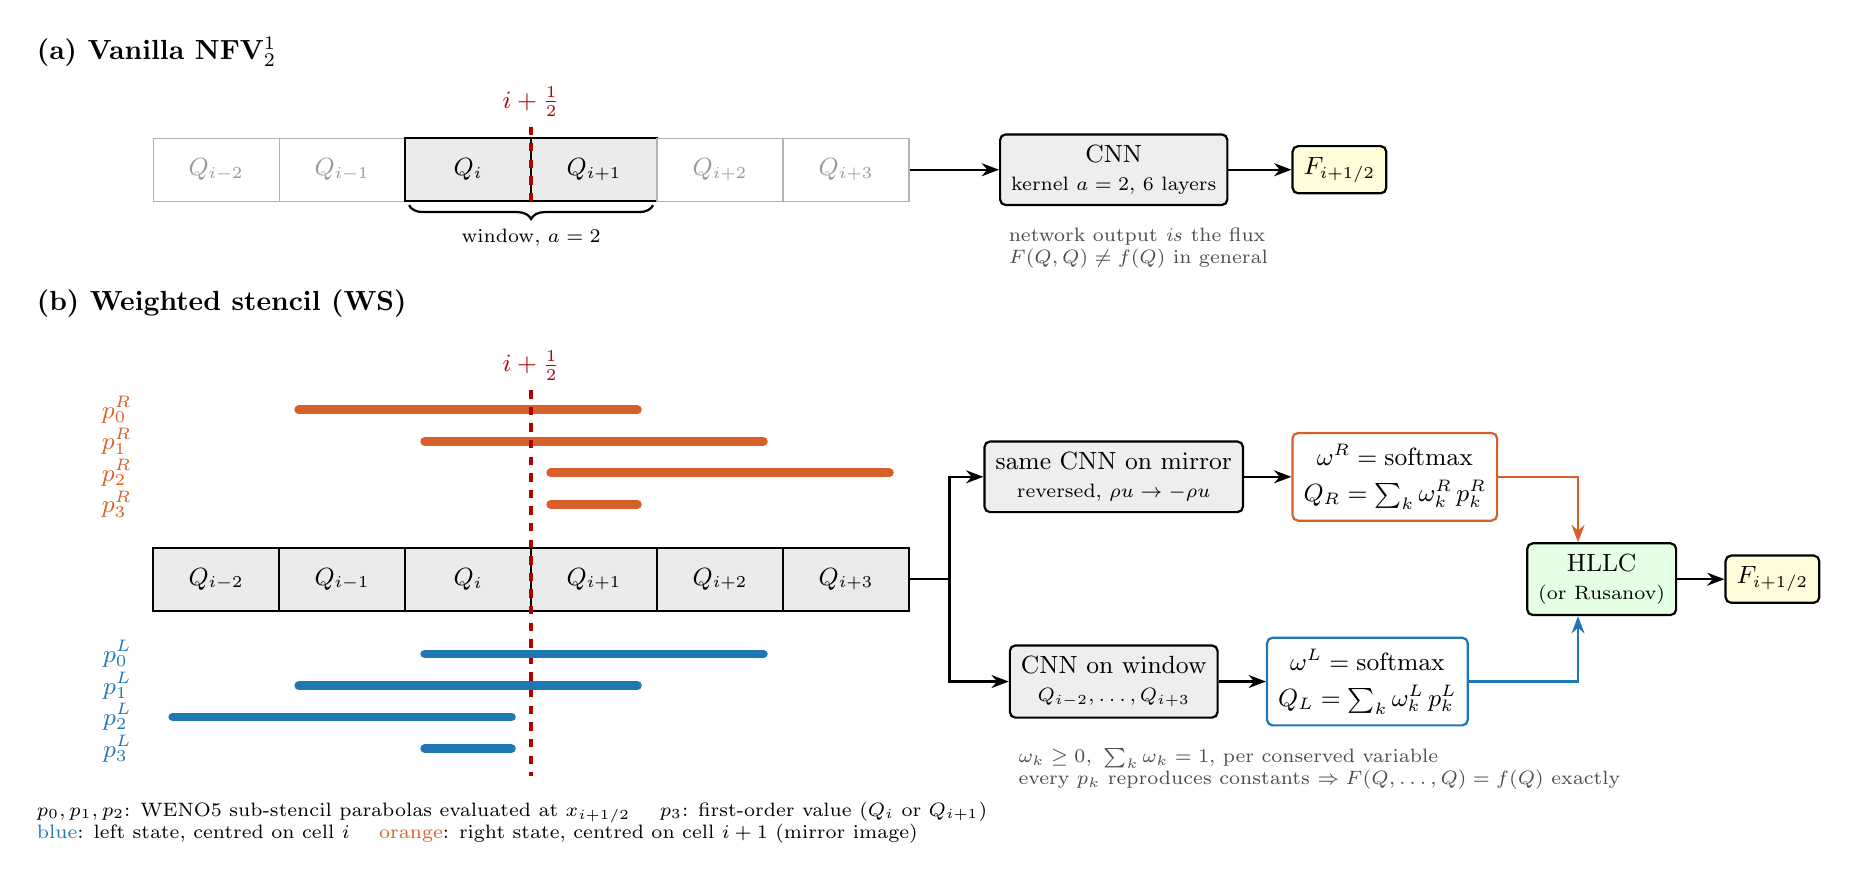
\begin{tikzpicture}

% ---------------- (a) vanilla NFV ----------------
\node[anchor=west, font=\bfseries] at (-1.6,4.1) {(a) Vanilla NFV$_2^1$};
\gdef\st{off}
\row{2.6}{2,3}{a}
\draw[face] (4.8,2.2) -- (4.8,3.15);
\node[red!70!black, font=\small, above] at (4.8,3.15) {$i+\tfrac12$};

\node[box, fill=cN!10] (cnnA) at (12.2,2.6) {CNN\\[-1pt]\scriptsize kernel $a=2$, 6 layers};
\node[box, fill=yellow!15, right=0.8cm of cnnA] (FA) {$F_{i+1/2}$};
\draw[decorate, decoration={brace, amplitude=5pt, mirror}, thick] (3.25,2.15) -- (6.35,2.15)
  node[midway, below=5pt, font=\scriptsize] {window, $a=2$};
\draw[arr] (a5.east) -- (cnnA);
\draw[arr] (cnnA) -- (FA);
\node[font=\scriptsize, align=left, anchor=north west, text=black!70] at ($(cnnA.south west)+(0,-0.15)$)
  {network output \emph{is} the flux\\ $F(Q,Q)\neq f(Q)$ in general};

% ---------------- (b) weighted stencil ----------------
\node[anchor=west, font=\bfseries] at (-1.6,0.9) {(b) Weighted stencil (WS)};

% right-state candidates (above the row), centred on cell i+1
\cand{1}{3}{-0.45}{cR}{$p^R_0$}
\cand{2}{4}{-0.85}{cR}{$p^R_1$}
\cand{3}{5}{-1.25}{cR}{$p^R_2$}
\cand{3}{3}{-1.65}{cR}{$p^R_3$}

\row{-2.6}{0,1,2,3,4,5}{b}
\draw[face] (4.8,-0.2) -- (4.8,-5.1);
\node[red!70!black, font=\small, above] at (4.8,-0.2) {$i+\tfrac12$};

% left-state candidates (below the row), centred on cell i
\cand{2}{4}{-3.55}{cL}{$p^L_0$}
\cand{1}{3}{-3.95}{cL}{$p^L_1$}
\cand{0}{2}{-4.35}{cL}{$p^L_2$}
\cand{2}{2}{-4.75}{cL}{$p^L_3$}

% pipeline
\node[box, fill=cN!10] (cnnL) at (12.2,-3.9) {CNN on window\\[-1pt]\scriptsize $Q_{i-2},\dots,Q_{i+3}$};
\node[box, fill=cN!10] (cnnR) at (12.2,-1.3) {same CNN on mirror\\[-1pt]\scriptsize reversed, $\rho u \to -\rho u$};
\node[box, draw=cL, right=0.6cm of cnnL] (QL) {$\omega^L=\mathrm{softmax}$\\[2pt] $Q_L=\sum_k \omega^L_k\,p^L_k$};
\node[box, draw=cR, right=0.6cm of cnnR] (QR) {$\omega^R=\mathrm{softmax}$\\[2pt] $Q_R=\sum_k \omega^R_k\,p^R_k$};
\node[box, fill=green!10] (rs) at ($(QL.east)!0.5!(QR.east)+(1.5,0)$) {HLLC\\[-1pt]\scriptsize (or Rusanov)};
\node[box, fill=yellow!15, right=0.6cm of rs] (FB) {$F_{i+1/2}$};

\draw[arr] (b5.east) -- ++(0.5,0) |- (cnnL.west);
\draw[arr] (b5.east) -- ++(0.5,0) |- (cnnR.west);
\draw[arr] (cnnL) -- (QL);
\draw[arr] (cnnR) -- (QR);
\draw[arr, cL] (QL.east) -| ($(rs.south)+(-0.3,0)$);
\draw[arr, cR] (QR.east) -| ($(rs.north)+(-0.3,0)$);
\draw[arr] (rs) -- (FB);

\node[font=\scriptsize, align=left, anchor=north west, text=black!70] at ($(cnnL.south west)+(0,-0.25)$)
  {$\omega_k\ge 0,\ \sum_k\omega_k=1$, per conserved variable\\
   every $p_k$ reproduces constants $\Rightarrow F(Q,\dots,Q)=f(Q)$ exactly};

% legend for candidates
\node[font=\scriptsize, align=left, anchor=north west] at (-1.6,-5.3)
  {$p_0,p_1,p_2$: WENO5 sub-stencil parabolas evaluated at $x_{i+1/2}$ \quad
   $p_3$: first-order value ($Q_i$ or $Q_{i+1}$)\\
   {\color{cL}blue}: left state, centred on cell $i$ \quad
   {\color{cR}orange}: right state, centred on cell $i+1$ (mirror image)};

\end{tikzpicture}
\end{document}
